\documentclass[english,aps,prl]{revtex4}
\usepackage[T1]{fontenc}
\usepackage[latin9]{inputenc}
\usepackage{amstext}
\usepackage{graphicx}

\makeatletter
%%%%%%%%%%%%%%%%%%%%%%%%%%%%%% Textclass specific LaTeX commands.
\@ifundefined{textcolor}{}
{%
 \definecolor{BLACK}{gray}{0}
 \definecolor{WHITE}{gray}{1}
 \definecolor{RED}{rgb}{1,0,0}
 \definecolor{GREEN}{rgb}{0,1,0}
 \definecolor{BLUE}{rgb}{0,0,1}
 \definecolor{CYAN}{cmyk}{1,0,0,0}
 \definecolor{MAGENTA}{cmyk}{0,1,0,0}
 \definecolor{YELLOW}{cmyk}{0,0,1,0}
 }

%%%%%%%%%%%%%%%%%%%%%%%%%%%%%% User specified LaTeX commands.
\makeatother

\usepackage{babel}

\begin{document}

\title{Readout Line Filter}

\author{Daniel Sank} \affiliation{University of California Santa Barbara}

\date{April 2013}

\maketitle

\section{Notation}
Any time I am making a transformation from series to parallel circuits I use $Q_e$ as the $Q$ of the transformation. This $Q$ is generally frequency dependent. Characteristic impedances of resonance modes are noted with a superscript $^0$. For example, $Z_{rr}^0$ indicates the characteristic impedance of the readout resonator. Note that this is \emph{not} the transmission line characteristic impedance, but rather $\sqrt{L/C}$ where $L$ and $C$ are the equivalent inductance and capacitance of the resonance.

\section{Dependencies}
This calculation makes frequent use of parallel to series equivalence transformations. These transformations are explained in detail in my writeup posted on the theory section of the TWiki.

\section{Complete circuit}

The complete Purcell filter circuit is shown in Figure \ref{Fig:1}. We want to compute the damping imposed on the qubit by the readout resonator and filter circuitry. This is done by computing the resistive load presented to the qubit by the readout circuitry. The calculation proceeds in three steps. First we reduce the filter to a frequency dependent effective resistance. We then transform the readout resonator and filter resistance into an effective resistance shunting the qubit. Finally, we compute the $Q$ of the qubit due to this shunting resistance.

\begin{figure}
\begin{centering}
\includegraphics[width=9cm]{figure1.pdf} 
\par\end{centering}
\caption{The complete Purcell filtered readout circuit}
\label{Fig:1}
\end{figure}

\section{Impedance looking into filter}

\begin{figure}
\begin{centering}
\includegraphics[width=9cm]{figure2.pdf} 
\par\end{centering}
\caption{Reduction of the external load and filter. a) The series capacitance and resistance are transformed to a resistance in parallel with the filter. b) We keep the resistive part of the filter impedance. This leaves the readout resonator with a series capacitor and resistor shunt to ground.}
\label{Fig:2}
\end{figure}

We model the filter as an $LC$ resonator capacitively coupled to an external environmental resistance. In order to find the impedance of the filter we need to transform the series capacitor $C_e$ and resistor $R_e$ into a parallel equivalent. The $Q$ of the series circuit is \begin{eqnarray}
Q_e &=& \frac{1}{\omega R_e C_e} \\
&=& \frac{\omega_0}{\omega} \frac{1}{\omega_0 R_e C_e} \\
&=& \frac{1}{x} Q_e(\omega_0) \end{eqnarray}
where here $x\equiv \omega/\omega_0$ and $\omega_0$ is the resonance frequency of the filter. Using the transformation rules from my writeup on series/parallel equivalence we get the equivalent parallel resistance \begin{equation}
R_p(\omega) = R_e Q_e(\omega)^2 = R_e \frac{1}{x^2}Q_e(\omega_0)^2 = R_p(\omega_0)/x^2 \end{equation}
The filter with this effective parallel resistance in shown in Figure \ref{Fig:2} a.

Using this frequency dependent resistance we can get the impedance looking into the filter through basic circuit analysis. The result is \begin{equation}
Z_F = \frac{Q_F Z_F^0}{x^2 + iQ_F x - iQ_F/x} \end{equation}
where $x\equiv \omega/\omega_0$ and $Q_F$ is the \emph{on-resonance} $Q$ of the filter. The resistive part of this impedance is \begin{equation}
Z_F = \frac{Q_F Z_F^0}{1+2\delta x + i2Q_F \delta x + (1-iQ_F)\delta x^2}
\end{equation}
where we've expanded the denominator in powers of $\delta x \equiv x-1$. Keeping only first order terms of $\delta x$ the resistive part becomes \begin{equation}
\Re Z_F(\delta x) = Q_F Z_F^0 \frac{1+2\delta x}{(1+2\delta x)^2 + (2Q_F \delta x)^2} \end{equation}
The circuit with the filter reduced to this single frequency dependent resistance is shown in Figure \ref{Fig:2} b.

\section{Loading of readout resonator}

\begin{figure}
\begin{centering}
\includegraphics[width=9cm]{figure3.pdf} 
\par\end{centering}
\caption{Reduction of the readout resonator. a) The series $RC$ shunt is transformed into an equivalent parallel resistance. b) We take only the resistive part of the readout resonator impedance. This leaves a series capacitor and resistor shunting the qubit.}
\label{Fig:3}
\end{figure}

Now consider the impedance looking into $C_{\kappa}$. If we make the (not necessarily good) assumption that the reactance of $C_{\kappa}$ is a lot bigger than the reactance of the filter, then we can ignore the reactance of the filter. This leaves us with a series capacitor and resistor shunting the readout resonator. This is the same problem we just analyzed so we use the same method. The $Q$ of the transformation is \begin{eqnarray}
Q_e &=& \frac{1}{\omega R_F(\omega) C_{\kappa}} \\
&=& \frac{1}{\omega_0 R_F(\omega_0) C_{\kappa}} \frac{R_F(\omega_0)}{R_F(\omega)} \frac{1}{x} \\
&=& \frac{1}{x}\frac{R_F(\omega_0)}{R_F(\omega)} Q_e(\omega_0) \end{eqnarray}
The equivalent parallel resistance is therefore \begin{equation}
R_p(\omega) = R_F(\omega)Q_e(\omega)^2 = \frac{1}{x^2}R_p(\omega_0) \left( \frac{R(\omega_0)}{R(\omega)}\right) \end{equation}
The circuit with this effective parallel resistance incorporated into the readout resonator is shown in Figure \ref{Fig:3} a. With this result we can compute the impedance looking into the readout resonator \begin{eqnarray}
Z_{rr}(\omega) &=& \frac{Z_{rr}^0 Q_{rr}}{x^2 \frac{R(\omega)}{R(\omega_0)} +iQ_{rr}x - iQ_{rr}/x} \\
&=& \frac{Z_{rr}^0 Q_{rr}}{x^2 \frac{1+2\delta x}{(1+2\delta x)^2+(2 Q_F \delta x)^2} +iQ_{rr}x - iQ_{rr}/x} \\
&\approx&  \frac{Z_{rr}^0 Q_{rr}}{\frac{1+4\delta x}{(2 Q_F \delta x)^2} +i2Q_{rr}\delta x} \end{eqnarray}
The resistive part is \begin{eqnarray}
R_{rr}(\omega) &=& \frac{Z_{rr}^0Q_{rr}}{\frac{1+4\delta x}{(2Q_F \delta x)^2} + \frac{(2Q_F\delta x)^2(2Q_{rr}\delta x)^2}{1+4\delta x}} \\
&\approx& \frac{Z_{rr}^0Q_{rr}(1+4\delta x)}{(2Q_F\delta x)^2(2Q_{rr}\delta x)^2} \end{eqnarray}
We have now reduced the circuit to a series capacitor and resistor shunting the qubit, as shown in Figure \ref{Fig:3} b.

\section{Loading of qubit}
We now compute the loaded $Q$ of the qubit. This is given by \begin{equation}
Q_q = \frac{C_q}{C_g} Q_e \end{equation}
where $Q_e$ is the $Q$ of the loading circuit. In this case we have \begin{eqnarray}
Q_e &=& \frac{1}{\omega_q C_g R_{rr}(\omega_q)} \\
&=& \frac{4Q_F^2Q_{rr}^2\delta x^4}{\omega_q C_g Z_{rr}^0 Q_{rr} (1+4\delta x)} \end{eqnarray}
Plugging in for $Q_q$ \begin{eqnarray}
Q_q &=& \frac{C_q}{C_g}4Q_F^2Q_{rr} \frac{1}{\omega_q C_g Z_{rr}^0}\frac{\delta x^4}{1+4\delta x}\\
&=& \left( \frac{C_q}{C_g}\right)^2 4Q_F^2 Q_{rr} \frac{Z_q}{Z_{rr}^0}\frac{\delta x^4}{1+4\delta x} \end{eqnarray}
This equation uses the effective resonance impedance of the readout resonator, in our lumped model. The relation between this and the actual line impedance is \begin{equation}
Z_{rr}^0 = \frac{4}{\pi}Z_0 \end{equation}
yielding \begin{equation}
Q_q = \left( \frac{C_q}{C_g}\right)^2 \pi Q_F^2 Q_{rr} \frac{Z_q}{Z_0}\frac{\delta x^4}{1+4\delta x} \end{equation}

This appears to underestimate the $T_1$ we find with SPICE by almost exactly $\pi$.

\section{Simpler analysis}

A simpler analysis can be done by making approximations from the outset rather than iteratively as we work through the stages of the circuit. The essential assumptions is that the coupling capacitors all have higher impedance than the filter and readout resonators shunting to ground. This is expected to be a good assumption, since at the qubit frequency we are off resonance from the resonators.

We start with the definition of $Q$ \begin{equation}
Q_q = \frac{\textrm{Energy stored in qubit}} {\textrm{energy lost per radian}} = \omega_q \frac{\textrm{Energy stored in qubit}}{\textrm{Power loss in }R_e} = \omega_q \frac{\frac{1}{2}C_qV_q^2}{\frac{1}{2}V_e^2/R_e} = \omega_q R_eC_q \left| V_q/V_e \right|^2 \label{eq:qubitQ} \end{equation}
To compute the ratio $V_q/V_e$ we use voltage division. With a voltage $V_q$ across the qubit, and assuming $Z_g \gg Z_{rr}$ we have a current $I = V_q/Z_g$ flowing through $C_g$. The voltage accross the readout resonator is therefore $IZ_{rr}=\frac{V_q Z_{rr}}{Z_g}$. Using similar arguments to work through each stage we arrive at \begin{equation}
\frac{V_e}{V_q} = \frac{R Z_F Z_{rr}}{Z_e Z_{\kappa} Z_g} \label{eq:voltageRatio} \end{equation}
Note all the shunt impedances in the numerator and the series capacitor impedances in the denominator.

Next we find the frequency dependence of $Z_{rr}$ and $Z_F$. We model these as lossless parallel $LC$ circuits. The impedance is then \begin{equation}
Z = \frac{-i\omega L}{2\delta x + \delta x^2} \approx \frac{-iZ_{LC}}{2\delta x + \delta x^2}\end{equation}
Here $Z_{LC}$ is the characteristic impedance of the equivalent $LC$ circuit for each of our $\lambda/4$ resonators. It is not equal to the line impedance of the resonators. Substituting this into equation (\ref{eq:voltageRatio}) and keeping lowest order terms in $\delta x$ we get \begin{equation}
\frac{V_e}{V_q} = -\frac{1}{4\delta x^2}\frac{R_e Z_F^0 Z_{rr}^0}{Z_e Z_{\kappa} Z_g} \end{equation}

We need to remove $Z_F^0$ and $Z_{rr}^0$ in favor of the $Q$ values of those two resonators. Using the results from \footnote{My loaded mode writeup} we can easily find the $Q$ of the filter \begin{equation}
Q_F = \frac{|Z_e|^2}{R_e |Z_F^0|} \end{equation}
To find the $Q$ of the readout resonator note that the filter can now be regarded as a \emph{lossy} resonator. Since the readout resonator and filter have similar resonance frequencies we can take the filter impedance to be its on-resonance value, which is \emph{real} and equal to $Q_F Z_F^0$. This is illustrated in figure ??. Using the same formula as for the filter we can write down the $Q$ of the readout resonator \begin{equation}
Q_{rr} = \frac{|Z_{\kappa}|^2}{Q_F Z_F^0 |Z_{rr}^0|} \end{equation}
Substituting these $Q$'s into equation (\ref{eq:voltageRatio}) we get \begin{equation}
\left| \frac{V_e}{V_q} \right| = \frac{1}{Q_F} \sqrt{\frac{R_e |Z_{rr}^0|}{Q_{rr}}} \frac{1}{|Z_g|} \frac{1}{4\delta x^2} \end{equation}
and substituting this into equation (\ref{eq:qubitQ}) we get \begin{equation}
Q_q = \frac{\omega_q C_q |Z_g|^2}{|Z_{rr}^0|} Q_F^2 Q_{rr} 16 \delta x^4 \end{equation}
Noting that the coupling capacitor impedances must be computed \emph{at the qubit frequency} we can put $|Z_g|=1/\omega_q C_g$. Also using $Z_q^0 = 1/\omega_q C_q$ we get \begin{equation}
Q_q = \left(\frac{C_q}{C_g}\right)^2 \frac{|Z_q^0|}{|Z_{rr}^0|} Q_F^2 Q_{rr} 16 \delta x^4 \end{equation}
Using the fact that for the $\lambda /4$ resonator the resonance characteristic impedance is equal to $4/\pi$ times the line impedance we finally get \begin{equation}
Q_q = 4\pi \left(\frac{C_q}{C_g}\right)^2 \frac{|Z_q^0|}{Z_0} Q_F^2 Q_{rr} \delta x^4 \end{equation}
Note that is is larger than the previous calculation by a factor of 4. Since the previous one was almost exactly $\pi$ lower than what we found in SPICE I think this second calculation is better and I made a mistake in the other one.

This can be re-expressed as \begin{equation}
T_1 = 4Q_F^2 \frac{1}{\kappa_{rr}} \frac{\Delta^4}{g^2 f_{rr}f_q} = 4Q_F^2 \left(\frac{\Delta^2}{f_q f_{rr}}\right) \frac{1}{\kappa_{rr}} \left(\frac{\Delta}{g}\right)^2 = 4 Q_F^2 \left(\frac{\Delta^2}{f_q f_{rr}}\right) T_1^{\textrm{(no filter)}} \end{equation}
This result is slightly different from what Eyob got.

\subsection{Result in absence of filter}

Using exactly the same method we can compute the damping expected in a case without a filter \begin{equation}
Q = \pi \left( \frac{C_q}{C_g} \right)^2 \frac{Z_q^0}{Z_0} Q_{rr} \delta x^2 \end{equation}
This can be rewritten as \begin{equation}
T_1 = \frac{1}{\kappa} \left( \frac{\Delta}{g} \right)^2 \end{equation}
Here $\kappa$ is the energy decay rate of the resonator equal to $2\pi f / Q$, and $g$ is the coupling between the qubit and resonator expressed as a frequency (dimensions of 1/time). This is the standard formula.

\end{document}